% Luonnolliset luvut esitellään nyt kokonaislukujen alussa.

% \sivulaatikko{engl. \emph{natural numbers, counting numbers} ruots. \emph{naturliga tal}}
% 
% 
% \laatikko{Luonnollisia lukuja käytetään kolmeen eri tarkoitukseen:
% 
% \begin{enumerate}
% \item Lukumäärien ilmoittamiseen (kardinaaliluvut)
% \item Järjestyksen ilmoittamiseen (ordinaaliluvut)
% \item Indeksointiin ja asioiden nimeämiseen
% \end{enumerate}
% }


% \section{Tehtäviä}
% 
% \begin{tehtava}
% 
% Onko kardinaali vai ordinaali vai indeksointi?
% 
% \end{tehtava}

\chapter{Kokonaisluvut}

Yksinkertaisimmat käyttämämme luvut ovat lukumäärien ilmaisemiseen käytetyt $0, 1, 2, 3, \ldots$. Näitä kutsutaan \emph{luonnollisiksi luvuiksi}, ja niiden joukkoa eli kaikkia luonnollisia lukuja yhdessä merkitään symbolilla $\mathbb{N}$.
%Edellä nolla määriteltiin luonnolliseksi luvuksi, mutta tästä ei ole yhteistä sopimusta: jotkut pitävät nollaa luonnollisena lukuna ja toiset eivät.

Luonnollisille luvuille $m$ ja $n$ on määritelty yhteenlasku $m + n$, esimerkiksi $5 + 3 = 8$.

Luonnollisten lukujen $m$ ja $n$ kertolasku määritellään peräkkäisinä yhteenlaskuina
\[m \cdot n = \underbrace{m + m + \ldots + m}_{n\text{ kpl}} = \underbrace{n + n + \ldots + n}_{m\text{ kpl}}.\]

\laatikko{
Nollalla kertomisen ajatellaan olevan "tyhjä yhteenlasku"\ eli nolla,
\[0 \cdot m = 0\].
}

Luonnollisten lukujen $m$ ja $n$ erotus määritellään yhteenlaskun avulla:
$m-n$ on luku $k$, jolle $k + n = m$. Kahden luonnollisen luvun erotus
ei kuitenkaan aina ole luonnollinen luku, esimerkkinä $3 - 5$.
Ratkaisemme ongelman määrittelemällä kullekin luonnolliselle
luvulle $n$ vastaluvun $-n$, jolle $n + (-n) = 0$.

Luonnolliset luvut ja niiden vastaluvut muodostavat yhdessä
kokonaislukujen joukon
\[\mathbb{Z} = \{\ldots, -2, -1, 0, 1, 2, \ldots\}.\]
Kun käytämme kokonaislukuja, voidaan kahden luvun erotus määritellä
yhteenlaskun ja vastaluvun avulla yksinkertaisesti $m-n = m+(-n)$.



\section{Yhteen- ja vähennyslasku}

    Kysymys: Mitä saadaan, kun luvusta $5$ vähennetään luku $-8$?
    
    \laatikko{
        Määritelmä
        
        Jokaisella luvulla $a$ on vastaluku $-a$, jolle pätee $a+(-a)=0$.
    }
    
    Esimerkiksi luvun $2$ vastalukua merkitään $-2$, ja sille pätee $2+(-2)=0$. Vastaavasti luvun $-2$ vastaluku on sellainen luku, joka laskettuna yhteen luvun $-2$ kanssa antaa luvun $0$. Tämä on tietysti $2$, koska $-2+2=0$. Näin voidaan huomata, että $-(-2)=2$.
    
    Negatiivisten ja positiivisten lukujen yhteen- ja vähennyslaskut voidaan myös tulkita lukusuoran avulla.
    
    % tässä on vähän kyseenalaista käyttää sekaisin sanallista ja numeerista esitystä
    
    $5+8$ "viiteen lisätään kahdeksan"
    \begin{center}
    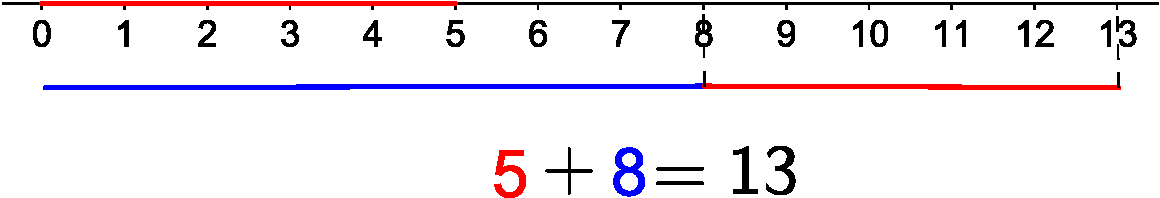
\includegraphics[scale=0.5]{01-luvut/kuvia/5plus8on13-crop.pdf}
    \end{center}
    
    $5+(+8)$ "viiteen lisätään plus kahdeksan"
    
    $+8$ tarkoittaa samaa kuin $8$. '$+$'-merkkiä käytetään luvun edessä silloin, kun halutaan korostaa, että kyseessä on nimenomaan positiivinen luku.
    
    \begin{center}
    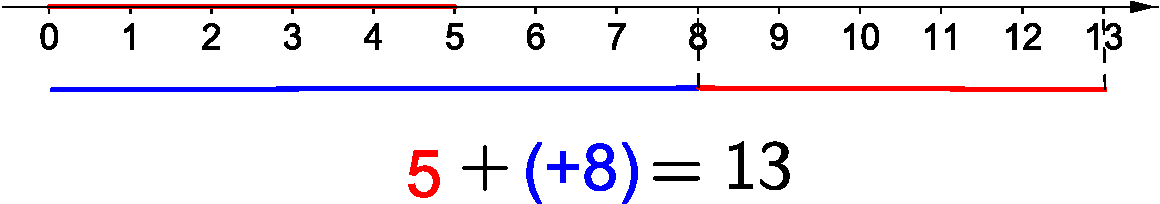
\includegraphics[scale=0.5]{01-luvut/kuvia/5plusplus8on13-crop.pdf}
    \end{center}
    
    $5-(+8)$ "viidestä vähennetään $+8$"
    
    Tämä tarkoittaa samaa kuin 5-8. Lukusuoralla siis liikutaan 8 pykälää taaksepäin.
    
    \begin{center}
    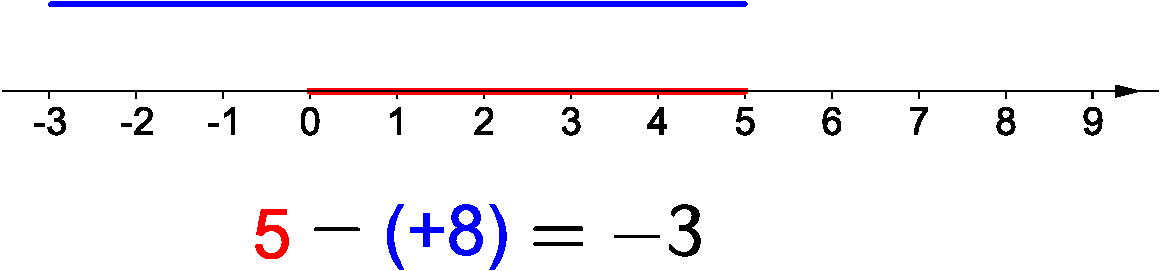
\includegraphics[scale=0.5]{01-luvut/kuvia/5miinusplus8onmiinus3-crop.pdf}
    \end{center}
    
    Mitä tapahtuu, kun lisätään negatiivinen luku? Kun lukuun lisätään $1$, se kasvaa yhdellä. Kun lukuun lisätään $0$, se ei kasva lainkaan. Kun lukuun lisätään negatiivinen luku, esim. $-1$, on luonnollista ajatella, että se pienenee. Tällä logiikalla negatiivisen luvun lisäämisen pitäisi siis pienentää alkuperäistä lukua. Siksi on sovittu, että $5+(-8)$ on yhtä suuri kuin $5-8$.
    
    \begin{center}
    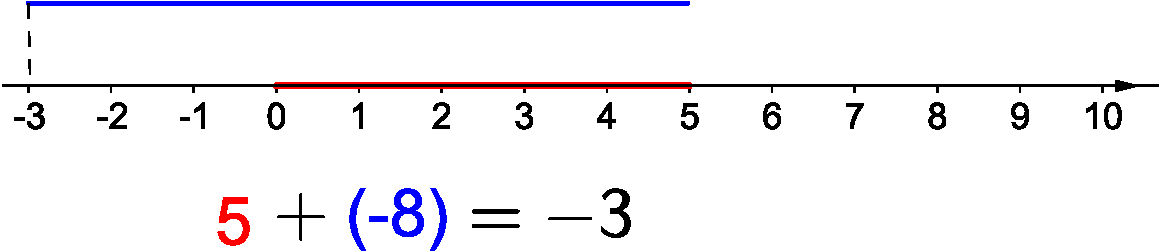
\includegraphics[scale=0.5]{01-luvut/kuvia/5plusmiinus8onmiinus3-crop.pdf}
    \end{center}
    
    $5-(-8)$ "viidestä vähennetään miinus kahdeksan"
    
    Negatiivisen luvun lisääminen on vastakohta positiivisen luvun lisäämiselle. Tällöin on luonnollista, että negatiivisen luvun vähentäminen on vastakohta positiivisen luvun vähentämiselle. Koska positiivisen luvun vähentäminen pienentää lukua, pitäisi negatiivisen luvun vähentämisen kasvattaa lukua. Tämän vuoksi on sovittu, että $5-(-8)$ tarkoittaa samaa kuin $5+8$.
    
    \begin{center}
    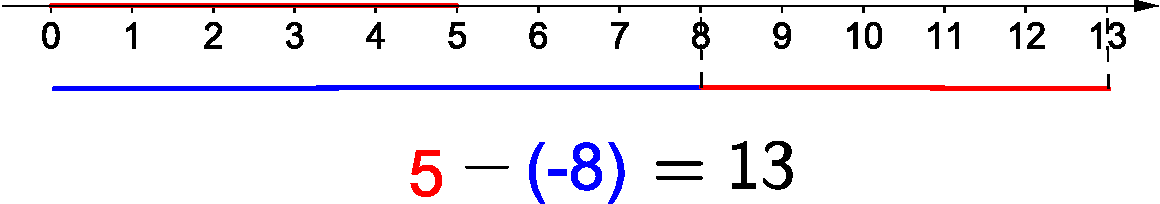
\includegraphics[scale=0.5]{01-luvut/kuvia/5miinusmiinus8on13-crop.pdf}
    \end{center}
    
    Samaan logiikkaan perustuen on sovittu myös merkkisäännöt positiivisten ja negatiivisten lukujen kertolaskuissa. Kun negatiivinen ja positiivinen luku kerrotaan keskenään, saadaan negatiivinen luku, mutta kun kaksi negatiivista lukua kerrotaan keskenään, saadaan positiivinen luku.

\section{Kertolasku}

    $3 \cdot 4$ "kolme kappaletta nelosia"
    
    \missingfigure{$3 \cdot 4$ lukusuoralla}
    
    $3 \cdot (-4)$ "kolme kappaletta miinus-nelosia"
    
    \missingfigure{$3 \cdot (-4)$ lukusuoralla}
    
    $-3 \cdot 4$ "miinus-kolme nelinkertaistetaan"
    
    \missingfigure{$-3 \cdot 4$ lukusuoralla}
    
    $-3 \cdot (-4)$ "miinus-kolme miinus-nelinkertaistetaan"
    
    \missingfigure{$-3 \cdot (-4)$ lukusuoralla}

\section{Jakolasku}

        Kun ensin kerrotaan jollain ja sitten jaetaan samalla luvulla, päädytään takaisin samaan, mistä lähdettiin.  Jakolaskujen merkkisäännöt on sovittu niin, että tämä ominaisuus säilyy. Ne ovat siis samat kuin kertolaskujen merkkisäännöt.
    
    Esimerkiksi haluamme, että $(-12):(-3)\cdot (-3)=-12$. Nyt voimme kysyä, mitä laskun $(-12):(-3)$ tulokseksi pitäisi tulla, jotta jakolasku ja kertolasku säilyvät toisilleen käänteisinä, eli mikä luku kerrottuna $-3$:lla on $-12$. Kertolaskun merkkisäännöistä nähdään helposti, että tämän luvun täytyy olla $+4$ eli $4$. Niinpä on sovittu, että $(-12):(-3)=12:3=4$.
    
\section{Yhteenveto}

\laatikko{
Laskusääntöjä
\begin{itemize}
\item $a-(-b)=a+b$
\item $-a\cdot (-b)=a\cdot b=ab$
\item $-a:(-b)=a: b=a:b$
\end{itemize}
}
    
    \section{Jaollisuus ja tekijöihinjako}

   
    \laatikko{
    Kokonaisluku $a$ on jaollinen kokonaisluvulla $b$, jos on olemassa kokonaisluku $c$ niin, että $a = b \cdot c$. Tällöin sanotaan myös, että $b$ on $a$:n tekijä.
    }
    
    \begin{esimerkki}
    \begin{enumerate}[a)]
    \item Luku $-12$ on jaollinen luvulla $3$:lla, sillä $-12 = 3 \cdot (-4)$.
    \item $-12$ ei ole jaollinen $5$:llä, sillä ei ole kokonaislukua, joka kerrottuna viidellä olisi $12$.
    \end{enumerate}
    \end{esimerkki}
    
    \missingfigure{Kuva, jossa on suorakaide, joka on jaettu 3x4 osaan.}
    
    Yllä jaollisuus määritellään kertolaskun avulla. Jaollisuuden voi määritellä myös jakolaskun avulla niin, että $a$ on jaollinen $b$:llä, mikäli $a:b$ on kokonaisluku. Esimerkiksi $12$ on jaollinen $3$:lla, koska $12:3 = 4$, joka on kokonaisluku.
    %Tämä määritelmä vaatii kuitenkin, että $b \neq 0$, joten sitä ei voida pitää yleispätevänä määritelmänä jaollisuudelle. Se on kuitenkin monesti yksinkertaisempi tapa ajatella.
   
    
    Kaikki luvut ovat jaollisia itsellään ja luvulla $1$. Esimerkiksi $7=7 \cdot 1=1 \cdot 7$, joten $7$ on jaollinen $1$:llä ja $37$:llä.
    
    \laatikko{
    \emph{Alkuluku} on ykköstä suurempi luku, joka on jaollinen ainoastaan luvulla $1$ ja itsellään.
    }
    
    Esimerkiksi luvut 2, 3, 5, 7, 11, 13, 17 ja 19 ovat alkulukuja. 
    
    \laatikko{
    \textbf{Aritmetiikan peruslause}
    
    Jokainen ykköstä suurempi kokonaisluku voidaan esittää yksikäsitteisesti alkulukujen tulona.
    }
    
    \todo{maininta siitä, todistetaanko aritmetiikan peruslause vai ei}
    
    Esimerkiksi luku $84$ voidaan kirjoittaa muodossa $2\cdot 2\cdot 3\cdot 7$. Kokeilemalla havaitaan, että 2, 3, ja 7 ovat kaikki alkulukuja. Aritmetiikan peruslauseen nojalla tiedetään, että tämä on ainoa tapa kirjoittaa $84$ alkulukujen tulona - mahdollista kertolaskujärjestyksen vaihtoa lukuunottamatta.
    
    %Kun luku $84$ esitetään muodossa $2\cdot 2\cdot 3\cdot 7$ on tapana sanoa, että se on \emph{jaettu alkutekijöihin}. Alkutekjät esitetään yleensä kasvavassa numerojärjestyksessä. Jos sama luku esiintyy tekijöissä useampaan kertaan, on se yleensä yleensä tapana merkitä potenssina. Tällöin luku $84$ voitaisiin kirjoittaa tekijöihin jaettuna $2^2\cdot 3\cdot 7$ ja luku $96$ muodossa $2\cdot 2\cdot 2\cdot 2\cdot 2\cdot 3=2^5\cdot 3$.
    
    %Luvun alkutekijät voi löytää etsimällä luvulle ensin jonkin esityksen kahden luvun tulona. Näiden kahden luvun ei tarvitse olla alkulukuja. Sen jälkeen sama toistetaan näille kahdelle luvulle ja edelleen aina uusille luvuille, kunnes tulossa on jäljellä vain alkulukuja.
    
    %\begin{esimerkki}
    %Luvun $96$ alkutekijät voi löytää vaikkapa seuraavanlaisella ketjulla: $96 = 2 \cdot 48 = 2 \cdot (2 \cdot 24) = 2 \cdot 2 \cdot (6 \cdot 4) = 2 \cdot 2 \cdot (2 \cdot 3) \cdot (2 \cdot 2)$. Nyt jäljellä on vain alkulukuja ja saatu tulo voidaan kirjoittaa lyhennettynä $96 = 2^5 \cdot 3$.
    %\end{esimerkki}
    
    \section*{Tehtäviä}
    
    
        \begin{tehtava}
        Kirjoita laskutoimitukseksi. (Laskuun ei tarvitse merkitä yksikköjä, eli celciusasteita tai euroja.)


        \begin{enumerate}[a)]
            \item Pakkasta on aluksi $-10 ^{\circ}$C, ja sitten se lisääntyy kahdella pakkasasteella.
            \item Pakkasta on aluksi $-20 ^{\circ}$C, ja sitten se hellittää (vähentyy) kolme (pakkas)astetta.
            \item Lämpötila on aluksi $17 ^{\circ}$C, ja sitten se vähentyy viisi astetta.
            \item Lämpötila on aluksi $5 ^{\circ}$C, ja sitten se kasvaa kuusi astetta.
            \item Mies on mafialle $30 000$ euroa velkaa ja menehtyy. Hänen kolme
                poikaansa jakavat velan tasan keskenään. Kuinka paljon kukin on
                velkaa mafialle? Merkitse velkaa negatiivisella luvulla.
        \end{enumerate}
        
        \begin{vastaus}
            \begin{enumerate}[a)]
                \item $-10+(-2)=-12$
                \item $-20-(-3)=-17$
                \item $17-5=12$
                \item $5+6=11$
                \item $\frac{-30 000}{3}=10 000$
            \end{enumerate}
        \end{vastaus}
    \end{tehtava}
    
    \begin{tehtava}
    Laske
    \begin{enumerate}[a)]
        \item $11+(-14)$
        \item $-8-(-4)$
        \item $-9-(+7)$
        \item $-(-8)+(5)-(-(-11))$
        \item $-8:(-4)$
        \item $(-8):(-4)$
        \item $(-5)\cdot 12$
    \end{enumerate}
        \begin{vastaus}
        \begin{enumerate}[a)]
            \item $2$
            \item $-3$
            \item $-4$
            \item $-16$
            \item $2$
            \item $2$
            \item $2$
            \item $-60$
        \end{enumerate}
        \end{vastaus}
    \end{tehtava}

    \begin{tehtava}
        Laske
        \begin{enumerate}[a)]
            \item $3+5$
            \item $10-5-6+1$
            \item $2 \cdot 2 - 1$
            \item $-9 - 5 \cdot (-2) + 3$
            \item $10 \cdot (5 - 2)$
            \item $(2-5)(5 - 1) + 1$
            \item $-9 - 2 \cdot ( 3 - 2 \cdot (3\cdot2 - 1))$
        \end{enumerate}

        \begin{vastaus}
            \begin{enumerate}[a)]
                \item $3$
                \item $0$
                \item $3$
                \item $4$
                \item $30$
                \item $-11$
                \item $5$
            \end{enumerate}
        \end{vastaus}
    \end{tehtava}

    \begin{tehtava}
    Mitkä seuraavista luvuista ovat jaollisia luvulla $4$? Jos luku $a$ on jaollinen luvulla $4$, kerro, millä kokonaisluvulla $b$ pätee $a = 4 \cdot b$.\\
    a) 1 \quad b) 12  \quad c) 13 \quad d) 2 \quad e) -20 \quad f) 0
    
    \begin{vastaus}
    \begin{enumerate}[a)]
    	\item Ei ole jaollinen luvulla 4
    	\item On jaollinen luvulla 4, $12 = 4 \cdot 3$
    	\item Ei ole jaollinen luvulla 4
    	\item Ei ole jaollinen luvulla 4
    	\item On jaollinen luvulla 4, $-20 = 4 \cdot (-5)$
    	\item On jaollinen luvulla 4, $0 = 4 \cdot 0$
    \end{enumerate}
    \end{vastaus}
    \end{tehtava}
    
    \begin{tehtava}
    Mitkä seuraavista luvuista ovat alkulukuja? Jos luku ei ole alkuluku, esitä se joidenkin kahden kokonaisluvun (jotka eivät ole ykkönen ja luku itse) tulona.\\
    a) 6 \quad b) 11 \quad c) 29 \quad d) -27 \quad e) -11 \quad f) 0
    
    \begin{vastaus}
    \begin{enumerate}[a)]
    	\item Ei ole alkuluku, esim. $6 = 2 \cdot 3$
    	\item On alkuluku
    	\item On alkuluku
    	\item Ei ole alkuluku, esim. $27 = 3 \cdot (-9)$
    	\item Ei ole alkuluku, esim. $-11 = (-1) \cdot 11$ Huom. alkuluvut ovat suurempia kuin yksi (ja siis positiivisia)
    	\item Ei ole alkuluku, esim. $0 = 6 \cdot 0$
    \end{enumerate}
    \end{vastaus}
    \end{tehtava}
    
    
    \begin{tehtava}
    Jaa seuraavat luvut alkutekijöihin.\\
    a) 12 \quad b) 15 \quad c) 28 \quad d) 30 \quad e) 64 \quad f) 90 \quad g) 100
    
    \begin{vastaus}
    \begin{enumerate}[a)]
    	\item $12 = 2^2 \cdot 3$
    	\item $15 = 3 \cdot 5$
    	\item $28 = 2^2 \cdot 7$
    	\item $30 = 2 \cdot 3 \cdot 5$
    	\item $64 = 2^6$
    	\item $90 = 2 \cdot 3^2 \cdot 5$
    	\item $100 = 2^2 \cdot 5^2$
    \end{enumerate}
    \end{vastaus}
    \end{tehtava}